\documentclass{article}
\usepackage{amsmath}
\usepackage{algorithm}
\usepackage[a4paper, margin=0.8in]{geometry}
\usepackage{algpseudocode}
\usepackage{graphicx}
\usepackage{amssymb}
\usepackage{pifont}
\usepackage{tikz}
\usetikzlibrary{calc}
\usetikzlibrary{positioning}
\usepackage{float}
\usepackage{caption}
\usepackage{abstract}
\usepackage{makeidx}
\makeindex

\setlength{\parskip}{0.5cm}
\setlength{\parindent}{0pt}

\title{Disjoint Sets}
\author{Mohammed Rizin \\ Umemployed}
\date{\today}

\begin{document}
\maketitle
% \printindex

\section{Disjoint sets \& operations} 
\index{Disjoint sets \& operations}
This is similar to the concept from sets in Mathematics but not exactly same. Disjoint set is modified for its proper usage in creating algorithms. The famous algorithm based on disjoint set is criskell's algorithm.

There are two main operation in a disjoint set:
\begin{enumerate}
\item Find
\item Join
\end{enumerate}

Lets us find How we can do 

\begin{center} \label{fig1}
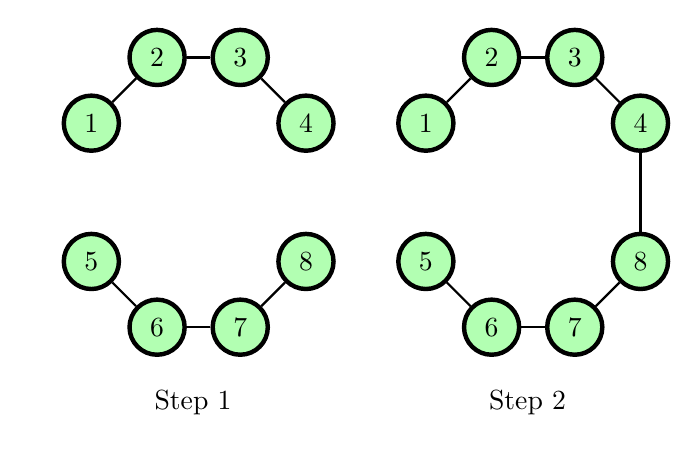
\begin{tikzpicture}[roundnode/.style={circle, draw=black, fill = green!30 , ultra thick, minimum size = 7mm}, sibling distance = 2mm]
    %Nodes
    \node[rectangle] (step1) {};
    % First step
    \node[roundnode] (node1) [below right=3mm and 3mm of step1] {1};
    \node[roundnode] (node2) [above right=3mm and 3mm of node1] {2};
    \node[roundnode] (node3) [right=3mm of node2] {3};
    \node[roundnode] (node4) [below right=3mm and 3mm of node3] {4};

    \draw[-, thick] (node1) -- (node2);
    \draw[-, thick] (node2) -- (node3);
    \draw[-, thick] (node3) -- (node4);

    \node[roundnode] (node5) [below=of node1] {5};
    \node[roundnode] (node6) [below right=3mm and 3mm of node5] {6};
    \node[roundnode] (node7) [right=3mm of node6] {7};
    \node[below=3mm of node7, xshift=-6mm] {Step 1};
    \node[roundnode] (node8) [above right=3mm and 3mm of node7] {8};

    \draw[-, thick] (node5) -- (node6);
    \draw[-, thick] (node6) -- (node7);
    \draw[-, thick] (node7) -- (node8);

    % Second step
    \node[rectangle] (step2) [right=4cm of step1] {};
    \node[roundnode] (node1b) [below right=3mm and 3mm of step2] {1};
    \node[roundnode] (node2b) [above right=3mm and 3mm of node1b] {2};
    \node[roundnode] (node3b) [right=3mm of node2b] {3};
    \node[roundnode] (node4b) [below right=3mm and 3mm of node3b] {4};

    \draw[-, thick] (node1b) -- (node2b);
    \draw[-, thick] (node2b) -- (node3b);
    \draw[-, thick] (node3b) -- (node4b);

    \node[roundnode] (node5b) [below=of node1b] {5};
    \node[roundnode] (node6b) [below right=3mm and 3mm of node5b] {6};
    \node[roundnode] (node7b) [right=3mm of node6b] {7};
    \node[below=3mm of node7b, xshift=-6mm] {Step 2};
    \node[roundnode] (node8b) [above right=3mm and 3mm of node7b] {8};

    \draw[-, thick] (node5b) -- (node6b);
    \draw[-, thick] (node6b) -- (node7b);
    \draw[-, thick] (node7b) -- (node8b);
    \draw[-, thick] (node4b) -- (node8b); % Added connection

\end{tikzpicture}
\captionof{figure} {Sample Graph}
\end{center}

First we can represent them as two sets:
\begin{align*}
    S_1 &= \left\{ 1, 2, 3, 4 \right\} \\
    S_2 &= \left\{ 5, 6, 7, 8 \right\} \\
    \text{Now }&\text{ we connect the  edge (4, 8)} \\
    S_1 &= \{ 1, 2, 3, \underbrace{4}_{\cdot} \} \\
    S_2 &= \{ 5, 6, 7, \underbrace{8}_{\cdot} \} \\
    \text{Both}&\text{ are in different set Create the Union of two sets}\\
    S_3 &= S_1 \cup S_2 = \{1, 2, 3, 4, 5, 6, 7, 8 \} \\
\end{align*}

\section{Detecting a cycle} \index{Detecting a cycle}
\begin{center} \label{fig2}
    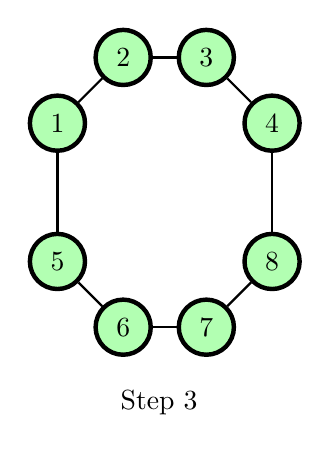
\begin{tikzpicture}[roundnode/.style={circle, draw=black, fill = green!30 , ultra thick, minimum size = 7mm}, sibling distance = 2mm]
        \node[roundnode] (node1c) {1};
        \node[roundnode] (node2c) [above right=3mm and 3mm of node1c] {2};
        \node[roundnode] (node3c) [right=3mm of node2c] {3};
        \node[roundnode] (node4c) [below right=3mm and 3mm of node3c] {4};
    
        \draw[-, thick] (node1c) -- (node2c);
        \draw[-, thick] (node2c) -- (node3c);
        \draw[-, thick] (node3c) -- (node4c);
    
        \node[roundnode] (node5c) [below=of node1c] {5};
        \node[roundnode] (node6c) [below right=3mm and 3mm of node5c] {6};
        \node[roundnode] (node7c) [right=3mm of node6c] {7};
        \node[below=3mm of node7c, xshift=-6mm] {Step 3};
        \node[roundnode] (node8c) [above right=3mm and 3mm of node7c] {8};
    
        \draw[-, thick] (node5c) -- (node6c);
        \draw[-, thick] (node6c) -- (node7c);
        \draw[-, thick] (node7c) -- (node8c);
        \draw[-, thick] (node4c) -- (node8c); % Added connection
        \draw[-, thick] (node1c) -- (node5c); % Added connection
    
    \end{tikzpicture}
    \captionof{figure} {Sample Graph}
    \end{center}

In Figure, we considered one more edge between 1 and 5. When we search for those elements and find which set it belong to, we end up finding same set for both the values. Hence, It's a cycle. If both the elements of an edge is found to in same set, then We say that the graph has a cycle.


\textbf{Confusion : Most of them would be confused we Union operation}\\
In mathematics, we do union between sets just as operation. But in here we have a purpose of doing the operation. Let me explain it!\\
If there is an edge between $(u, v)  |  u, v \in \mathcal{G}$, check which set does $u$ and $v$ belong to different set $S_1$ and $S_2$ will connect each other. Once they are connected, we perform union operation. Still Daunting actually!\\
Lets me explain more simply.\\
\begin{align*}
    \text{Initially }&\text{ we have two sets } S_1 = \{1, 2, 3, 4\} \text{ and } S_2 = \{5, 6, 7, 8\} \\
    \text{Now }&\text{ we connect the  edge (4, 8)} \\
    S_1 &= \{ 1, 2, 3, \underbrace{4}_{\cdot} \} \\
    S_2 &= \{ 5, 6, 7, \underbrace{8}_{\cdot} \} \\
    \text{Both}&\text{ are in different set Create the Union of two sets}\\
    S_3 &= S_1 \cup S_2 = \{1, 2, 3, 4, 5, 6, 7, 8 \} \\
\end{align*}

When we have an edge between $u$ and $v$, Why do we perform union, why not any other operation?\\
Hmm...! Let me put it in another way to make it more clear.\\
One of the most plausible reason I could come up is. Once we join the two sets, every elements of set $S_1$ can be accessed by the elements of $S_2$ and vice versa. Maybe I should get okay with this explanation. Haha!



\section{Graphical Representation} \index{Graphical Representation}
Now let create another graph and see how we can represent it in a disjoint set.\\
\begin{center} \label{fig2}
    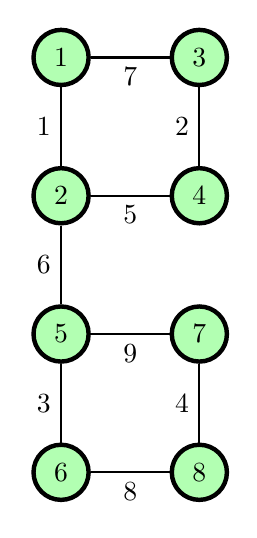
\begin{tikzpicture}[roundnode/.style={circle, draw=black, fill = green!30 , ultra thick, minimum size = 7mm}, sibling distance = 2mm]
        \node[roundnode] (node1) {1};
        \node[roundnode] (node2) [below=of node1] {2};
        \node[roundnode] (node3) [right=of node1] {3};
        \node[roundnode] (node4) [below=of node3] {4};
        \node[roundnode] (node5) [below=of node2] {5};
        \node[roundnode] (node7) [right=of node5] {7};
        \node[roundnode] (node6) [below=of node5] {6};
        \node[roundnode] (node8) [right=of node6] {8};
        

        \draw[-, thick] (node1) -- (node2) node[midway, auto, swap] {$1$};
        \draw[-, thick] (node1) -- (node3) node[midway, auto, swap] {$7$};
        \draw[-, thick] (node3) -- (node4) node[midway, auto, swap] {$2$};
        \draw[-, thick] (node2) -- (node4) node[midway, auto, swap] {$5$};

        \draw[-, thick] (node2) -- (node5) node[midway, auto, swap] {$6$};
        \draw[-, thick] (node5) -- (node6) node[midway, auto, swap] {$3$};
        \draw[-, thick] (node5) -- (node7) node[midway, auto, swap] {$9$};
        \draw[-, thick] (node7) -- (node8) node[midway, auto, swap] {$4$}; 
        \draw[-, thick] (node6) -- (node8) node[midway, auto, swap] {$8$};
    \end{tikzpicture}
\captionof{figure} {Sample Graph}
\end{center}

\begin{enumerate}
    \item At first we have n singletons sets: $\{1\}, \{2\}, \{3\}, \{4\}, \{5\}, \{6\}, \{7\}, \{8\}$
    \item Now we connect the edge 1 (1, 2) i.e., sets $\{1\}$ and $\{2\}$, so we perform Union $\{1, 2\}$. 1 is the parent of 2.
    \item Then we connect the edge 2 (3, 4) i.e., sets $\{3\}$ and $\{4\}$, so we perform Union $\{3, 4\}$. 3 is the parent of 4.
    \item Then we connect the edge 3 (5, 6) i.e., sets $\{5\}$ and $\{6\}$, so we perform Union $\{5, 6\}$. 5 is the parent of 6.
    \item Then we connect the edge 4 (7, 8) i.e., sets $\{7\}$ and $\{8\}$, so we perform Union $\{7, 8\}$. 7 is the parent of 8.
    \item Then we connect the edge 5 (2, 4) i.e., sets $\{1, 2\}$ and $\{3, 4\}$, so we perform Union $\{1, 2, 3, 4\}$.\\ 1 is the parent of 2 and 3 is the parent of 4 or 3 is the parent of 4 and 1 is the parent of 2. We choose 1 as root in this case.
    \item Then we connect the edge 6 (2, 5) i.e., sets $\{1, 2, 3, 4\}$ and $\{5, 6\}$, so we perform Union $\{1, 2, 3, 4, 5, 6\}$. 1 is the parent of 2 and 3 is the parent of 4 and 5 is the parent of 6. 
    \item Finally, we connect the edge 7 (1, 3). Both are in the same set. Hence, a cycle is detected. 
\end{enumerate}



\begin{center} \label{fig2}
    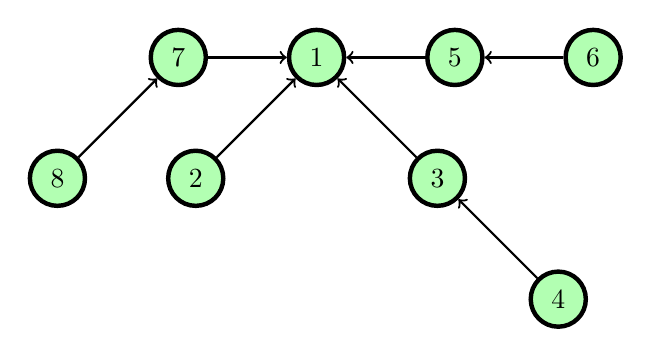
\begin{tikzpicture}[roundnode/.style={circle, draw=black, fill = green!30 , ultra thick, minimum size = 7mm}, sibling distance = 2mm]
        \node[roundnode] (node1) {1};
        \node[roundnode] (node2) [below left=of node1] {2};
        \node[roundnode] (node3) [below right=of node1] {3};
        \node[roundnode] (node4) [below right=of node3] {4};
        \node[roundnode] (node5) [right=of node1] {5};
        \node[roundnode] (node6) [right=of node5] {6};
        \node[roundnode] (node7) [left=of node1] {7};
        \node[roundnode] (node8) [below left=of node7] {8};
        

        \draw[<-, thick] (node1) -- (node2);
        \draw[<-, thick] (node1) -- (node3);
        \draw[<-, thick] (node3) -- (node4);
        \draw[<-, thick] (node1) -- (node5);
        \draw[<-, thick] (node5) -- (node6);
        \draw[<-, thick] (node7) -- (node8); 
        \draw[<-, thick] (node1) -- (node7);
    \end{tikzpicture}
\captionof{figure} {Graphical Representation}
\end{center}



\section{Array Representation} \index{Array Representation}
\begin{center}
    \textbf{Initial Array:}
    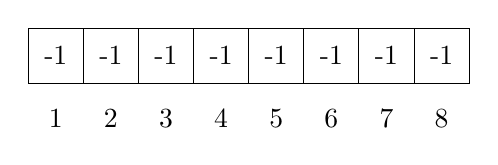
\begin{tikzpicture}[box/.style={rectangle, draw=black, minimum size=7mm}]
        \coordinate (A) at (0, 0);
        \def\A{-1, -1, -1, -1, -1, -1, -1, -1}
        \foreach \x[count=\i from 1] in \A
        {
            \node[box] at (A) {\x};
            \node at ($(A) - (0, 0.8)$) {\i};
            \coordinate (A) at ($(A) + (0.7, 0)$);
        }
    \end{tikzpicture}
\end{center}

\begin{enumerate}
    \item \textbf{Union(1, 2):}
    \begin{center}
        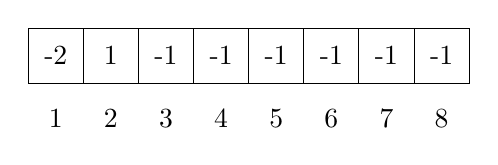
\begin{tikzpicture}[box/.style={rectangle, draw=black, minimum size=7mm}]
            \coordinate (A) at (0, 0);
            \def\A{-2, 1, -1, -1, -1, -1, -1, -1}
            \foreach \x[count=\i from 1] in \A
            {
                \node[box] at (A) {\x};
                \node at ($(A) - (0, 0.8)$) {\i};
                \coordinate (A) at ($(A) + (0.7, 0)$);
            }
        \end{tikzpicture}
    \end{center}

    \item \textbf{Union(3, 4):}
    \begin{center}
        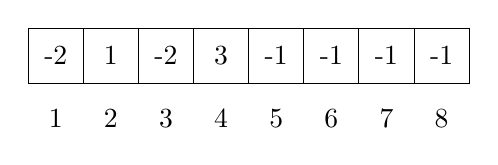
\begin{tikzpicture}[box/.style={rectangle, draw=black, minimum size=7mm}]
            \coordinate (A) at (0, 0);
            \def\A{-2, 1, -2, 3, -1, -1, -1, -1}
            \foreach \x[count=\i from 1] in \A
            {
                \node[box] at (A) {\x};
                \node at ($(A) - (0, 0.8)$) {\i};
                \coordinate (A) at ($(A) + (0.7, 0)$);
            }
        \end{tikzpicture}
    \end{center}

    \item \textbf{Union(5, 6):}
    \begin{center}
        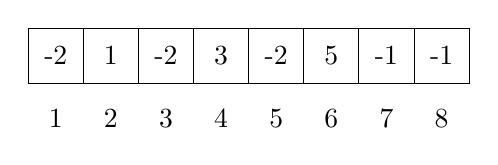
\begin{tikzpicture}[box/.style={rectangle, draw=black, minimum size=7mm}]
            \coordinate (A) at (0, 0);
            \def\A{-2, 1, -2, 3, -2, 5, -1, -1}
            \foreach \x[count=\i from 1] in \A
            {
                \node[box] at (A) {\x};
                \node at ($(A) - (0, 0.8)$) {\i};
                \coordinate (A) at ($(A) + (0.7, 0)$);
            }
        \end{tikzpicture}
    \end{center}

    \item \textbf{Union(7, 8):}
    \begin{center}
        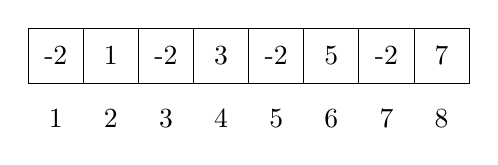
\begin{tikzpicture}[box/.style={rectangle, draw=black, minimum size=7mm}]
            \coordinate (A) at (0, 0);
            \def\A{-2, 1, -2, 3, -2, 5, -2, 7}
            \foreach \x[count=\i from 1] in \A
            {
                \node[box] at (A) {\x};
                \node at ($(A) - (0, 0.8)$) {\i};
                \coordinate (A) at ($(A) + (0.7, 0)$);
            }
        \end{tikzpicture}
    \end{center}

    \item \textbf{Union(2, 4):}
    \begin{center}
        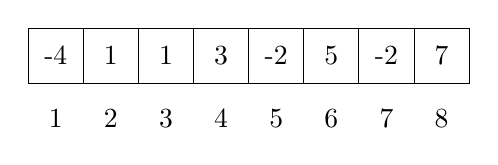
\begin{tikzpicture}[box/.style={rectangle, draw=black, minimum size=7mm}]
            \coordinate (A) at (0, 0);
            \def\A{-4, 1, 1, 3, -2, 5, -2, 7}
            \foreach \x[count=\i from 1] in \A
            {
                \node[box] at (A) {\x};
                \node at ($(A) - (0, 0.8)$) {\i};
                \coordinate (A) at ($(A) + (0.7, 0)$);
            }
        \end{tikzpicture}
    \end{center}

    \item \textbf{Union(2, 5):}
    \begin{center}
        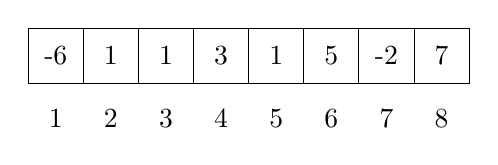
\begin{tikzpicture}[box/.style={rectangle, draw=black, minimum size=7mm}]
            \coordinate (A) at (0, 0);
            \def\A{-6, 1, 1, 3, 1, 5, -2, 7}
            \foreach \x[count=\i from 1] in \A
            {
                \node[box] at (A) {\x};
                \node at ($(A) - (0, 0.8)$) {\i};
                \coordinate (A) at ($(A) + (0.7, 0)$);
            }
        \end{tikzpicture}
    \end{center}

    \item \textbf{Union(1, 3):}
    \begin{center}
        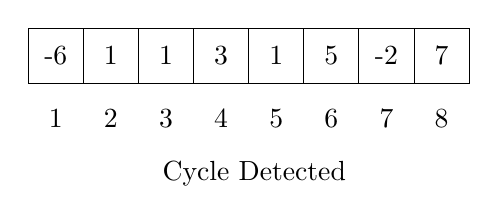
\begin{tikzpicture}[box/.style={rectangle, draw=black, minimum size=7mm}]
            \coordinate (A) at (0, 0);
            \def\A{-6, 1, 1, 3, 1, 5, -2, 7}
            \foreach \x[count=\i from 1] in \A
            {
                \node[box] at (A) {\x};
                \node at ($(A) - (0, 0.8)$) {\i};
                \coordinate (A) at ($(A) + (0.7, 0)$);
            }
            \node at ($0.45*(A) + (0, -1.5)$) {Cycle Detected};
        \end{tikzpicture}
    \end{center}
    \item \textbf{Union(6, 8):}
    \begin{center}
        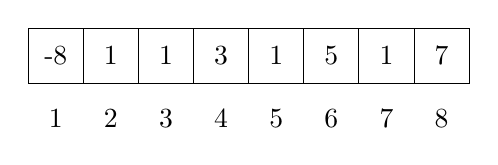
\begin{tikzpicture}[box/.style={rectangle, draw=black, minimum size=7mm}]
            \coordinate (A) at (0, 0);
            \def\A{-8, 1, 1, 3, 1, 5, 1, 7}
            \foreach \x[count=\i from 1] in \A
            {
                \node[box] at (A) {\x};
                \node at ($(A) - (0, 0.8)$) {\i};
                \coordinate (A) at ($(A) + (0.7, 0)$);
            }
        \end{tikzpicture}
    \end{center}

\begin{center} \label{fig2}
    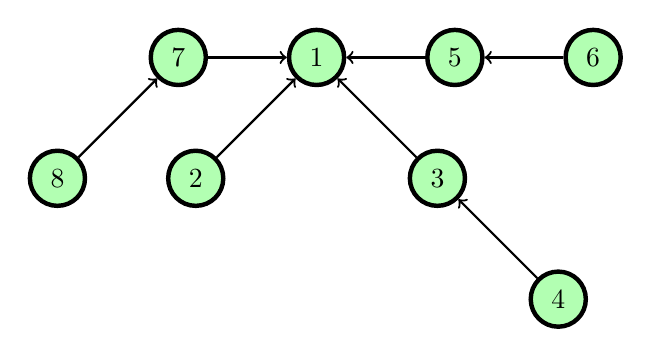
\begin{tikzpicture}[roundnode/.style={circle, draw=black, fill = green!30 , ultra thick, minimum size = 7mm}, sibling distance = 2mm]
        \node[roundnode] (node1) {1};
        \node[roundnode] (node2) [below left=of node1] {2};
        \node[roundnode] (node3) [below right=of node1] {3};
        \node[roundnode] (node4) [below right=of node3] {4};
        \node[roundnode] (node5) [right=of node1] {5};
        \node[roundnode] (node6) [right=of node5] {6};
        \node[roundnode] (node7) [left=of node1] {7};
        \node[roundnode] (node8) [below left=of node7] {8};
        

        \draw[<-, thick] (node1) -- (node2);
        \draw[<-, thick] (node1) -- (node3);
        \draw[<-, thick] (node3) -- (node4);
        \draw[<-, thick] (node1) -- (node5);
        \draw[<-, thick] (node5) -- (node6);
        \draw[<-, thick] (node7) -- (node8); 
        \draw[<-, thick] (node1) -- (node7);
    \end{tikzpicture}
\end{center}
\item \textbf{Union(5, 7):}
    \begin{center}
        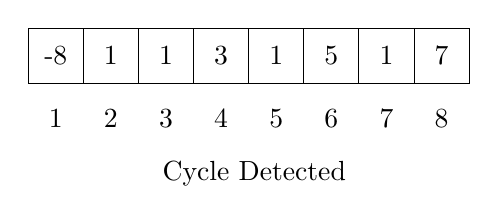
\begin{tikzpicture}[box/.style={rectangle, draw=black, minimum size=7mm}]
            \coordinate (A) at (0, 0);
            \def\A{-8, 1, 1, 3, 1, 5, 1, 7}
            \foreach \x[count=\i from 1] in \A
            {
                \node[box] at (A) {\x};
                \node at ($(A) - (0, 0.8)$) {\i};
                \coordinate (A) at ($(A) + (0.7, 0)$);
            }
            \node at ($0.45*(A) + (0, -1.5)$) {Cycle Detected};
        \end{tikzpicture}
    \end{center}

\end{enumerate}

\section{Weighted Union and collapsing Find} \index{Weighted Union and collapsing Find}

Weighted Union and collapsing Find are the two techniques used to optimize the disjoint set operations.\\
\begin{enumerate}
    \item \textbf{Weighted Union:} In this technique, we connect the smaller set to the larger set. This helps in reducing the height of the tree.\\
    \item \textbf{Collapsing Find:} In this technique, we make the parent of the node as the root of the tree. This helps in reducing the height of the tree.\\
\end{enumerate}

After applying the Weighted Union and collapsing Find techniques, the array representation will be as follows:\\
\begin{center}
    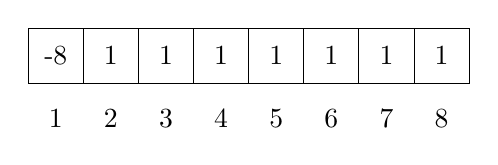
\begin{tikzpicture}[box/.style={rectangle, draw=black, minimum size=7mm}]
        \coordinate (A) at (0, 0);
        \def\A{-8, 1, 1, 1, 1, 1, 1, 1}
        \foreach \x[count=\i from 1] in \A
        {
            \node[box] at (A) {\x};
            \node at ($(A) - (0, 0.8)$) {\i};
            \coordinate (A) at ($(A) + (0.7, 0)$);
        }
    \end{tikzpicture}
\end{center}
and the graphical representation will be as follows:\\
\begin{center} \label{fig2}
    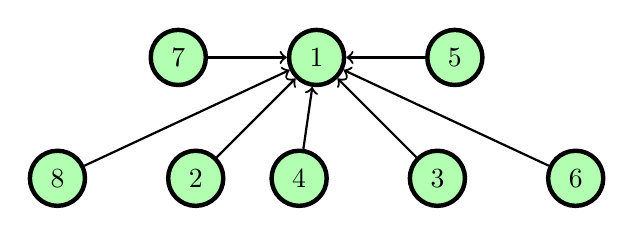
\begin{tikzpicture}[roundnode/.style={circle, draw=black, fill = green!30 , ultra thick, minimum size = 7mm}, sibling distance = 2mm]
        \node[roundnode] (node1) {1};
        \node[roundnode] (node2) [below left=of node1] {2};
        \node[roundnode] (node3) [below right=of node1] {3};
        \node[roundnode] (node4) [left=of node3] {4};
        \node[roundnode] (node5) [right=of node1] {5};
        \node[roundnode] (node6) [below right=of node5] {6};
        \node[roundnode] (node7) [left=of node1] {7};
        \node[roundnode] (node8) [below left=of node7] {8};
        

        \draw[<-, thick] (node1) -- (node2);
        \draw[<-, thick] (node1) -- (node3);
        \draw[<-, thick] (node1) -- (node4);
        \draw[<-, thick] (node1) -- (node5);
        \draw[<-, thick] (node1) -- (node6);
        \draw[<-, thick] (node1) -- (node8); 
        \draw[<-, thick] (node1) -- (node7);
    \end{tikzpicture}
\end{center}


\end{document}


